\documentclass{article}
\usepackage[a4paper, margin=2.5cm]{geometry}
\usepackage{amsmath}
\usepackage{caption}
\usepackage{placeins}
\usepackage{graphicx}
\usepackage{subcaption}
\usepackage{setspace}
\usepackage{float}

%\usepackage[active,tightpage]{preview}
\usepackage{natbib}
\bibpunct{(}{)}{,}{a}{}{;} 
\usepackage{url}
\usepackage{nth}
\usepackage{authblk}
% for the d in integrals
\newcommand{\dd}{\; \mathrm{d}}
\newcommand{\tc}{\quad\quad\text{,}}
\newcommand{\tp}{\quad\quad\text{.}}
\defcitealias{HMD}{HMD}

\newcommand\ackn[1]{%
  \begingroup
  \renewcommand\thefootnote{}\footnote{#1}%
  \addtocounter{footnote}{-1}%
  \endgroup
}
\begin{document}

%\title{Macro patterns in the shape of aging}
\title{Displaying changes in bivariate relationships over age and time}

\author[1]{Tim Riffe\thanks{riffe@demogr.mpg.de}}
\author[2]{Jos\'e Manuel Aburto \thanks{jmaburto@health.sdu.dk}}
\affil[1]{Max Planck Institute for Demographic Research}
\affil[2]{Epidemiology, Biostatistics and Biodemography, Department of Public Health, University of Southern Denmark}

\maketitle

\begin{abstract}
~
\begin{description}
\item[\textbf{Background}] Lexis surfaces are an established visualization
technique to show how a given value changes over age and time. Vector fields are
a two-dimensional representation of two variables: direction and speed (or
force). 
\item[\textbf{Objective}] We aim to increase the information density of patterns
shown on the Lexis surface by placing a vector field on the Lexis surface. 
\item[\textbf{Results}] We show Lexis fields using different combinations of
visual encodings, such as color, contour layering, and angle, length, curvature,
and thickness of field elements. These instruments enable information layering
that is not otherwise possible on standard Lexis surfaces.
\item[\textbf{Conclusions}] Lexis fields extend the analytic power of the Lexis
surface, and these can be rendered to display information at higher densities
than commonly made Lexis surfaces.
\end{description}
\end{abstract}


\section*{Introduction}
*map layering*
Maps in general combine layers of categorical, continuous, and
symbolic information projected onto a common set of spatial coordinates. Take
for example a weather map, which dispalys the extent of each level of storm
intensity with semitransparent color overlaid on a base map, which might
itself be a categorical partitioning of land uses, terrain types, including
a road network and place names. Atop the continuous or discrete representation
may be placed arrows depicting wind speed and direction, potentially colored in
to depict a hot or cold front.
eas Lexis maps, more commonly referred to as Lexis surfaces, are similar, but these more typically project a single continuous or categorical  Lexis surfaces are a graphical form used to display data on the Lexis coordinate plane, a Cartesian plane that is also a simplex relationship between age, period, and cohort. Surfaces are often displayed as heat maps, contours maps, perspective plots, or variants of these things. Various kinds of quantities, such as raw magnitudes, differences, ratios, intensities, proportions, derivatives, and even compositions \citep{scholey2017visualizing}) can be displayed on Lexis surfaces in order to put age, period, cohort, or other patterns in relief. 
Vector fields are a graphical form used to display variation in speed,
direction, or force over a plane. Point estimates of variation on the plane are
often represented with arrows where length is proportional to a function of
magnitude (force, speed) and where angle indicates direction. We propose a
fusion of these two graphical instruments, \emph{Lexis fields}, as a method to
display variation in relationships between variables over age and time. Our
example shows patterns in the relationship between remaining life expectancy and
the standard deviation of remaining lifespan over age and time based on all
available populations in the \citet{HMD} from 1950 onward. 



We offer several experimental variants of Lexis field design for our two
examples. The first of these, Figure~\ref{fig:sfig1}, is a bare-bones Lexis field that serves to illustrate the underlying concept. This display differs from a standard vector field in two notable ways. 1) Segments are drawn rather than arrows, because each slope can be
interpreted as a subplot, where the convention is to always read a
relationship from left to right. 2) The left and right extremes are fixed for
each segment according to the year-width rendered, in this case 5-year
groupings. This means that relationships farther from zero also result in longer
line segments, but the length of the line segment is not strictly proportional
to the magnitude of the slope coefficient or any other quantity. For each
subplot, the x range represents the same hypothetical range of
variation in remaining life expectancy or 2 years. The y-axis is arbitrarily,
but identically scaled for each subplot. Other criteria for slope length would
also be possible and will be considered.

Figure~\ref{fig:sfig2} is identical to the previous, but adds a red contour line
at the turning point in slopes. In this case there is only one sign change is slope
coefficients over the age pattern. It is easier to locate and detect change in
this (novel) threshold with the line markup than from the bare Lexis field.
Indeed one could add further isoclines at slope break points, as in
Figure~\ref{fig:sfig3} or \ref{fig:sfig4}, and insodoing we begin a transition
into the more standard graphical form of contour maps. Figure~\ref{fig:sfig3}
blends the Lexis field with a heatmap, where hue indicates both direction and
magnitude of slope coefficients. In this case, slope coefficients are
double-coded, and this display is likely the most legible, but it comes at a
cost of clutter. Figure~\ref{fig:sfig4} removes the slope segments, but is
otherwise identical. We wish to explore variants of the first three of these
Lexis field proposals, and may possibly display more example relationships
between other variables in a full manuscript, data permitting.

\begin{figure}
\begin{subfigure}{.5\textwidth}
  \centering
  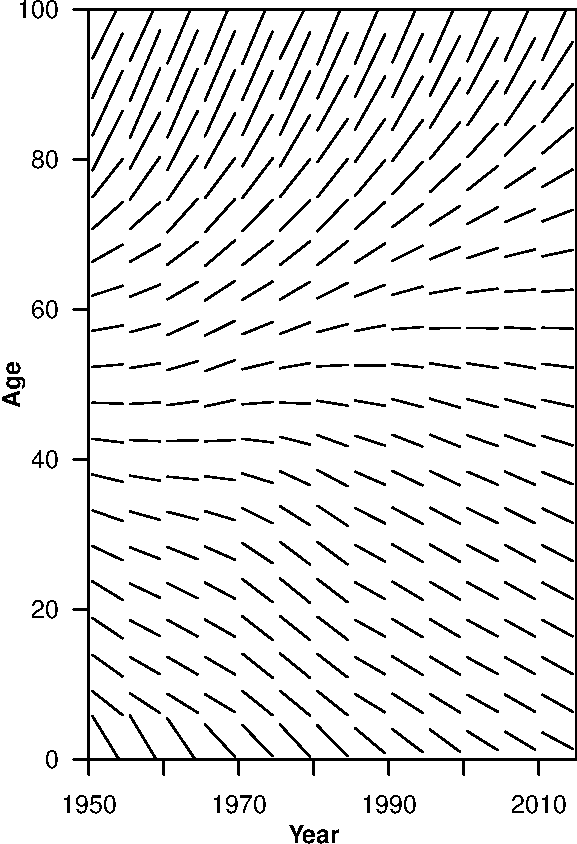
\includegraphics[scale=.6]{Figures/Fig9-crop.pdf}
  \caption{A simple field.}
  \label{fig:sfig1}
\end{subfigure}%
\begin{subfigure}{.5\textwidth}
  \centering
  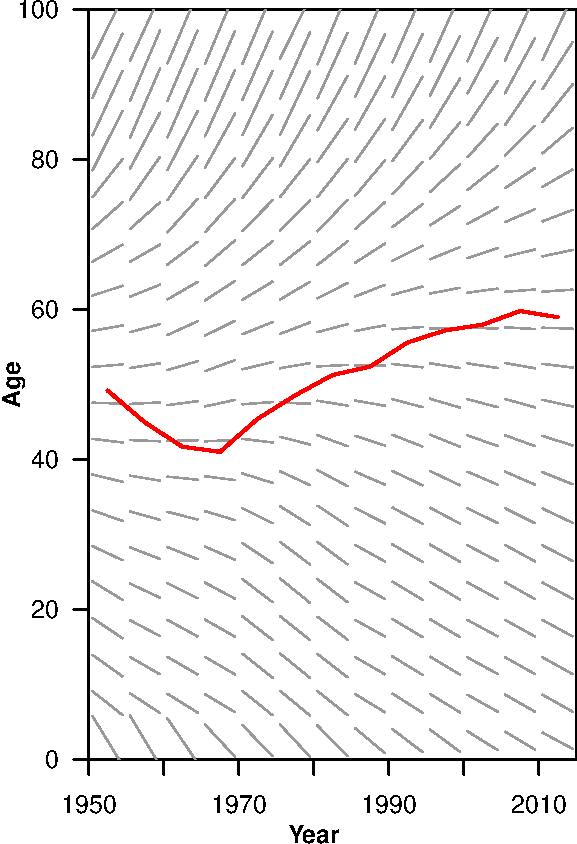
\includegraphics[scale=.6]{Figures/Fig10-crop.pdf}
  \caption{A simple field, with the zero-slope isocline drawn (red).}
  \label{fig:sfig2}
\end{subfigure}

\begin{subfigure}{.5\textwidth}
  \centering
  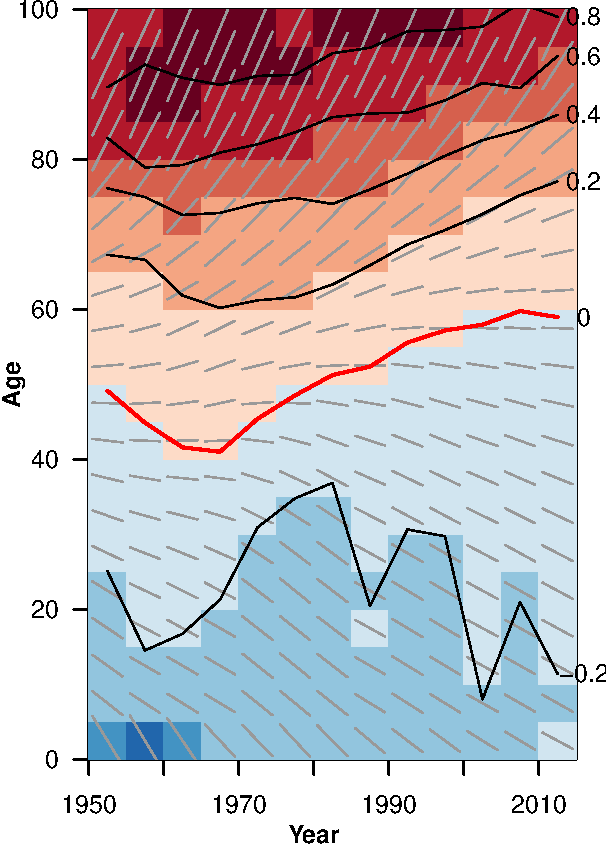
\includegraphics[scale=.6]{Figures/Fig11-crop.pdf}
  \caption{Slopes doubly coded with field segments and discrete color, further
  slope isoclines drawn.}
  \label{fig:sfig3}
\end{subfigure}%
\begin{subfigure}{.5\textwidth}
  \centering
  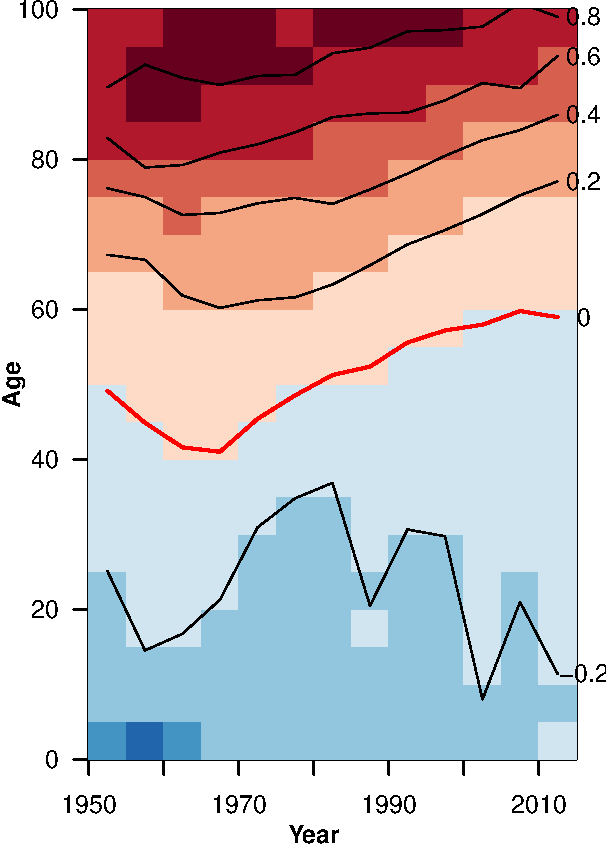
\includegraphics[scale=.6]{Figures/Fig12-crop.pdf}
  \caption{Discrete color heatmap with selected isoclines drawn.}
  \label{fig:sfig4}
\end{subfigure}
\caption{Four versions of Lexis fields displaying the linear
relationship between the standard deviation and mean of remaining
lifespan, males (HMD)}
\label{fig:fig}
\end{figure}



\nocite{vaupel1987thousands}

\FloatBarrier
\singlespacing
\bibliographystyle{plainnat}
  \bibliography{references} 

\end{document}
